% Created 2021-01-24 Sun 23:42
% Intended LaTeX compiler: pdflatex
\documentclass[11pt]{article}
\usepackage[utf8]{inputenc}
\usepackage[T1]{fontenc}
\usepackage{graphicx}
\usepackage{grffile}
\usepackage{longtable}
\usepackage{wrapfig}
\usepackage{rotating}
\usepackage[normalem]{ulem}
\usepackage{amsmath}
\usepackage{textcomp}
\usepackage{amssymb}
\usepackage{capt-of}
\usepackage{hyperref}
\usepackage{minted}
\hypersetup{colorlinks=true, linkcolor=black, filecolor=red, urlcolor=blue}
\usepackage[turkish]{babel}
\author{Eren Hatırnaz}
\date{24 Ocak 2021}
\title{Yazılım Gündemi\\\medskip
\large Haftalık yazılım gündemi değerlendirmesi}
\hypersetup{
 pdfauthor={Eren Hatırnaz},
 pdftitle={Yazılım Gündemi},
 pdfkeywords={},
 pdfsubject={},
 pdfcreator={Emacs 27.1 (Org mode 9.3)},
 pdflang={Turkish}}
\begin{document}

\maketitle
\shorthandoff{=}
\begin{center}
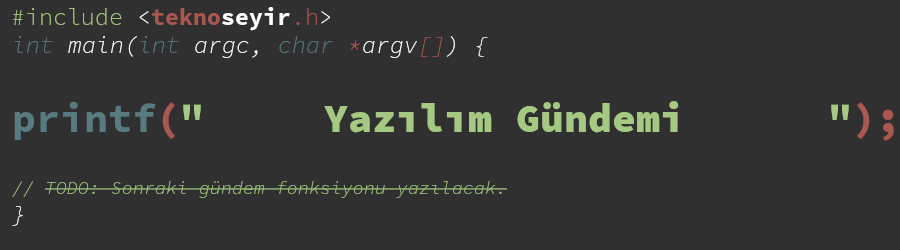
\includegraphics[width=.9\linewidth]{img/yazilim-gundemi-logo.png}
\end{center}

\section*{Nedir?}
\label{sec:orgb10dfbd}
Yazılım Gündemi, benim \href{https://teknoseyir.com/u/erenhatirnaz/blog}{TeknoSeyir Sosyal} platformunda 2019-2020 yılları
arasında her hafta düzenli olarak yazmaya çalıştığım bir yazı serisidir. Bu
yazı serisi kapsamında, her hafta, o hafta içerisinde programlamanın çeşitli
alanlarıyla ilgili internette karşılaştığım haberleri topluyordum. Topladığım
haberlerden ilgim ya da bilgim olanları detaylı değerlendiriyor; (b)ilgim
olmayanları ise "Diğer Haberler" başlığı altında listeliyordum. İlk yazılarda
olmasa da sonradan bir de "Yaklaşan Etkinlikler" bölümü ekledim. Bu bölümde de
bir sonraki hafta için planlanmış alanımızla ilgili bulabildiğim tüm
etkinlikleri tablo şeklinde veriyordum. Fakat hem biraz motivasyon kaybı
yaşadığım için hem de hayatımda farklı şeylere öncelik vermem gerektiği için
yazı serisine ara verdim.

Şunu da şöylemeliyim ki: Bu gündem yazıları o hafta içerisinde yazılım
dünyasında olan her şeyi kapsama garantisi vermiyor. Takip ettiğim
kaynaklarda karşıma çıkan güncel haberleri gündem yazıları içerisine
alıyordum. Takip ettiğim kaynakları aşağıdaki \hyperref[sec:orgb26d44d]{Kaynaklar} bölümünde
bulabilirsiniz.
\section*{Motivasyon}
\label{sec:org1dd7344}
TeknoSeyir'in en çok tükettiğim içerikleri Gündem Değerlendirmeleri
(teknoloji, oyun ve bilim). Her ne kadar teknoloji sektörünün içerisinden
birisi de olsam teknoloji gündemini o kadar sık takip edemiyorum. Aynı çekilde
bilim de ilgi alanım fakat onu da sürekli takip edebilecek bir vaktim yok.
TeknoSeyir'da hazırlanan bu içerikler tam olarak benim bu ihtiyaçlarımı
karşılıyor.

Benim sürekli takip ettiğim bir alan var, o da: Yazılım sektörü. Haftalık
Gündem Değerlendirmesi'nde her ne kadar yazılım sektörü içerisinden haberlere
sık sık yer verilse de, hitap ettiği kitleye doğal olarak uymadığından,
programlamanın daha içerisinden haberler pek fazla yer bulmuyordu. Ben de,
"madem kendim sürekli bu haberleri takip ediyorum, o halde neden ben böyle bir
içerik çıkartmayayım" dedim ve bu yazı serisini oluşturdum.

TeknoSeyir Sosyal'den birçok arkadaş bu yazı serisini podcast şeklinde sesli
bir içerik şeklinde hazırlamamı tavsiye ettiler, hatta şiddetle talep de
ettiler fakat ben kendimi yazarak daha iyi ifade edebildiğimi düşündüğüm için
girmedim o işlere. Ama günün birinde o yeteneklerimi de geliştirirsem neden
olmasın :).
\section*{Arşiv}
\label{sec:org9538b81}
Yazılım Gündemi yazılarının \textbf{HTML}, \textbf{PDF} ve \textbf{ORG} formatındaki sürümlerini
aşağıdaki listeden bulabilirsiniz.

\textbf{\textbf{Toplam gündem sayısı:}} 49

\textbf{\textbf{Toplam özel yazı sayısı:}} 1

\subsection*{2020}
\label{sec:org8bfe236}
\begin{center}
\begin{tabular}{lllll}
\hline
Yazılım Gündemi - 2020/26 & 29 Haziran - 5 Temmuz 2020 & \href{arsiv/2020/26/yazilim-gundemi-2020-26.html}{HTML} & \href{arsiv/2020/26/yazilim-gundemi-2020-26.pdf}{PDF} & \href{arsiv/2020/26/yazilim-gundemi-2020-26.pdf}{ORG}\\
Yazılım Gündemi - 2020/25 & 22-28 Haziran 2020 & \href{arsiv/2020/25/yazilim-gundemi-2020-25.html}{HTML} & \href{arsiv/2020/25/yazilim-gundemi-2020-25.pdf}{PDF} & \href{arsiv/2020/25/yazilim-gundemi-2020-25.pdf}{ORG}\\
Yazılım Gündemi - 2020/24 & 15-21 Haziran 2020 & \href{arsiv/2020/24/yazilim-gundemi-2020-24.html}{HTML} & \href{arsiv/2020/24/yazilim-gundemi-2020-24.pdf}{PDF} & \href{arsiv/2020/24/yazilim-gundemi-2020-24.pdf}{ORG}\\
Yazılım Gündemi - 2020/23 & 8-14 Haziran 2020 & \href{arsiv/2020/23/yazilim-gundemi-2020-23.html}{HTML} & \href{arsiv/2020/23/yazilim-gundemi-2020-23.pdf}{PDF} & \href{arsiv/2020/23/yazilim-gundemi-2020-23.pdf}{ORG}\\
Yazılım Gündemi - 2020/22 & 1-7 Haziran 2020 & \href{arsiv/2020/22/yazilim-gundemi-2020-22.html}{HTML} & \href{arsiv/2020/22/yazilim-gundemi-2020-22.pdf}{PDF} & \href{arsiv/2020/22/yazilim-gundemi-2020-22.pdf}{ORG}\\
Yazılım Gündemi - 2020/21 & 25-31 Mayıs 2020 & \href{arsiv/2020/21/yazilim-gundemi-2020-21.html}{HTML} & \href{arsiv/2020/21/yazilim-gundemi-2020-21.pdf}{PDF} & \href{arsiv/2020/21/yazilim-gundemi-2020-21.pdf}{ORG}\\
Yazılım Gündemi - 2020/20 & 18-24 Mayıs 2020 & \href{arsiv/2020/20/yazilim-gundemi-2020-20.html}{HTML} & \href{arsiv/2020/20/yazilim-gundemi-2020-20.pdf}{PDF} & \href{arsiv/2020/20/yazilim-gundemi-2020-20.pdf}{ORG}\\
Yazılım Gündemi - 2020/19 & 11-17 Mayıs 2020 & \href{arsiv/2020/19/yazilim-gundemi-2020-19.html}{HTML} & \href{arsiv/2020/19/yazilim-gundemi-2020-19.pdf}{PDF} & \href{arsiv/2020/19/yazilim-gundemi-2020-19.pdf}{ORG}\\
Yazılım Gündemi - 2020/18 & 4-10 Mayıs 2020 & \href{arsiv/2020/18/yazilim-gundemi-2020-18.html}{HTML} & \href{arsiv/2020/18/yazilim-gundemi-2020-18.pdf}{PDF} & \href{arsiv/2020/18/yazilim-gundemi-2020-18.pdf}{ORG}\\
Yazılım Gündemi - 2020/17 & 27 Nisan - 3 Mayıs 2020 & \href{arsiv/2020/17/yazilim-gundemi-2020-17.html}{HTML} & \href{arsiv/2020/17/yazilim-gundemi-2020-17.pdf}{PDF} & \href{arsiv/2020/17/yazilim-gundemi-2020-17.pdf}{ORG}\\
Yazılım Gündemi - 2020/16 & 20-26 Nisan 2020 & \href{arsiv/2020/16/yazilim-gundemi-2020-16.html}{HTML} & \href{arsiv/2020/16/yazilim-gundemi-2020-16.pdf}{PDF} & \href{arsiv/2020/16/yazilim-gundemi-2020-16.pdf}{ORG}\\
Yazılım Gündemi - 2020/15 & 13-19 Nisan 2020 & \href{arsiv/2020/15/yazilim-gundemi-2020-15.html}{HTML} & \href{arsiv/2020/15/yazilim-gundemi-2020-15.pdf}{PDF} & \href{arsiv/2020/15/yazilim-gundemi-2020-15.pdf}{ORG}\\
Yazılım Gündemi - 2020/14 & 6-12 Nisan 2020 & \href{arsiv/2020/14/yazilim-gundemi-2020-14.html}{HTML} & \href{arsiv/2020/14/yazilim-gundemi-2020-14.pdf}{PDF} & \href{arsiv/2020/14/yazilim-gundemi-2020-14.pdf}{ORG}\\
Yazılım Gündemi - 2020/13 & 30 Mart - 5 Nisan 2020 & \href{arsiv/2020/13/yazilim-gundemi-2020-13.html}{HTML} & \href{arsiv/2020/13/yazilim-gundemi-2020-13.pdf}{PDF} & \href{arsiv/2020/13/yazilim-gundemi-2020-13.pdf}{ORG}\\
Yazılım Gündemi - 2020/12 & 23-29 Mart 2020 & \href{arsiv/2020/12/yazilim-gundemi-2020-12.html}{HTML} & \href{arsiv/2020/12/yazilim-gundemi-2020-12.pdf}{PDF} & \href{arsiv/2020/12/yazilim-gundemi-2020-12.pdf}{ORG}\\
Yazılım Gündemi - 2020/11 & 16-22 Mart 2020 & \href{arsiv/2020/11/yazilim-gundemi-2020-11.html}{HTML} & \href{arsiv/2020/11/yazilim-gundemi-2020-11.pdf}{PDF} & \href{arsiv/2020/11/yazilim-gundemi-2020-11.pdf}{ORG}\\
Yazılım Gündemi - 2020/10 & 9-15 Mart 2020 & \href{arsiv/2020/10/yazilim-gundemi-2020-10.html}{HTML} & \href{arsiv/2020/10/yazilim-gundemi-2020-10.pdf}{PDF} & \href{arsiv/2020/10/yazilim-gundemi-2020-10.pdf}{ORG}\\
Yazılım Gündemi - 2020/09 & 2-8 Mart 2020 & \href{arsiv/2020/09/yazilim-gundemi-2020-09.html}{HTML} & \href{arsiv/2020/09/yazilim-gundemi-2020-09.pdf}{PDF} & \href{arsiv/2020/09/yazilim-gundemi-2020-09.pdf}{ORG}\\
Yazılım Gündemi - 2020/08 & 17 Şubat - 1 Mart 2020 & \href{arsiv/2020/08/yazilim-gundemi-2020-08.html}{HTML} & \href{arsiv/2020/08/yazilim-gundemi-2020-08.pdf}{PDF} & \href{arsiv/2020/08/yazilim-gundemi-2020-08.pdf}{ORG}\\
Yazılım Gündemi - 2020/07 & 10-16 Şubat 2020 & \href{arsiv/2020/07/yazilim-gundemi-2020-07.html}{HTML} & \href{arsiv/2020/07/yazilim-gundemi-2020-07.pdf}{PDF} & \href{arsiv/2020/07/yazilim-gundemi-2020-07.pdf}{ORG}\\
Yazılım Gündemi - 2020/06 & 3-9 Şubat 2020 & \href{arsiv/2020/06/yazilim-gundemi-2020-06.html}{HTML} & \href{arsiv/2020/06/yazilim-gundemi-2020-06.pdf}{PDF} & \href{arsiv/2020/06/yazilim-gundemi-2020-06.pdf}{ORG}\\
Yazılım Gündemi - 2020/05 & 27 Ocak - 2 Şubat 2020 & \href{arsiv/2020/05/yazilim-gundemi-2020-05.html}{HTML} & \href{arsiv/2020/05/yazilim-gundemi-2020-05.pdf}{PDF} & \href{arsiv/2020/05/yazilim-gundemi-2020-05.pdf}{ORG}\\
Yazılım Gündemi - 2020/04 & 20-26 Ocak 2020 & \href{arsiv/2020/04/yazilim-gundemi-2020-04.html}{HTML} & \href{arsiv/2020/04/yazilim-gundemi-2020-04.pdf}{PDF} & \href{arsiv/2020/04/yazilim-gundemi-2020-04.pdf}{ORG}\\
Yazılım Gündemi - 2020/03 & 13-19 Ocak 2020 & \href{arsiv/2020/03/yazilim-gundemi-2020-03.html}{HTML} & \href{arsiv/2020/03/yazilim-gundemi-2020-03.pdf}{PDF} & \href{arsiv/2020/03/yazilim-gundemi-2020-03.pdf}{ORG}\\
Yazılım Gündemi - 2020/02 & 6-12 Ocak 2020 & \href{arsiv/2020/02/yazilim-gundemi-2020-02.html}{HTML} & \href{arsiv/2020/02/yazilim-gundemi-2020-02.pdf}{PDF} & \href{arsiv/2020/02/yazilim-gundemi-2020-02.pdf}{ORG}\\
Yazılım Gündemi - 2020/01 & 1-5 Ocak 2020 & \href{arsiv/2020/01/yazilim-gundemi-2020-01.html}{HTML} & \href{arsiv/2020/01/yazilim-gundemi-2020-01.pdf}{PDF} & \href{arsiv/2020/01/yazilim-gundemi-2020-01.pdf}{ORG}\\
\hline
\end{tabular}
\end{center}
\subsection*{2019}
\label{sec:orgc5d7549}
\begin{center}
\begin{tabular}{lllll}
\hline
Yazılım Gündemi - 23 & 23-29 Aralık 2019 & \href{arsiv/2019/23/yazilim-gundemi-23.html}{HTML} & \href{arsiv/2019/23/yazilim-gundemi-23.pdf}{PDF} & \href{arsiv/2019/23/yazilim-gundemi-23.pdf}{ORG}\\
Yazılım Gündemi - 22 & 16-22 Aralık 2019 & \href{arsiv/2019/22/yazilim-gundemi-22.html}{HTML} & \href{arsiv/2019/22/yazilim-gundemi-22.pdf}{PDF} & \href{arsiv/2019/22/yazilim-gundemi-22.pdf}{ORG}\\
Yazılım Gündemi - 21 & 9-15 Aralık 2019 & \href{arsiv/2019/21/yazilim-gundemi-21.html}{HTML} & \href{arsiv/2019/21/yazilim-gundemi-21.pdf}{PDF} & \href{arsiv/2019/21/yazilim-gundemi-21.pdf}{ORG}\\
Yazılım Gündemi - 20 & 2-8 Aralık 2019 & \href{arsiv/2019/20/yazilim-gundemi-20.html}{HTML} & \href{arsiv/2019/20/yazilim-gundemi-20.pdf}{PDF} & \href{arsiv/2019/20/yazilim-gundemi-20.pdf}{ORG}\\
Yazılım Gündemi - 19 & 18 Kasım-1 Aralık 2019 & \href{arsiv/2019/19/yazilim-gundemi-19.html}{HTML} & \href{arsiv/2019/19/yazilim-gundemi-19.pdf}{PDF} & \href{arsiv/2019/19/yazilim-gundemi-19.pdf}{ORG}\\
Yazılım Gündemi - 18 & 11-17 Kasım 2019 & \href{arsiv/2019/18/yazilim-gundemi-18.html}{HTML} & \href{arsiv/2019/18/yazilim-gundemi-18.pdf}{PDF} & \href{arsiv/2019/18/yazilim-gundemi-18.pdf}{ORG}\\
Yazılım Gündemi - 17 & 4-10 Kasım 2019 & \href{arsiv/2019/17/yazilim-gundemi-17.html}{HTML} & \href{arsiv/2019/17/yazilim-gundemi-17.pdf}{PDF} & \href{arsiv/2019/17/yazilim-gundemi-17.pdf}{ORG}\\
Yazılım Gündemi - 16 & 28 Ekim - 3 Kasım 2019 & \href{arsiv/2019/16/yazilim-gundemi-16.html}{HTML} & \href{arsiv/2019/16/yazilim-gundemi-16.pdf}{PDF} & \href{arsiv/2019/16/yazilim-gundemi-16.pdf}{ORG}\\
Yazılım Gündemi - 15 & 21-27 Ekim 2019 & \href{arsiv/2019/15/yazilim-gundemi-15.html}{HTML} & \href{arsiv/2019/15/yazilim-gundemi-15.pdf}{PDF} & \href{arsiv/2019/15/yazilim-gundemi-15.pdf}{ORG}\\
Yazılım Gündemi - 14 & 14-20 Ekim 2019 & \href{arsiv/2019/14/yazilim-gundemi-14.html}{HTML} & \href{arsiv/2019/14/yazilim-gundemi-14.pdf}{PDF} & \href{arsiv/2019/14/yazilim-gundemi-14.pdf}{ORG}\\
Yazılım Gündemi - 13 & 7-13 Ekim 2019 & \href{arsiv/2019/13/yazilim-gundemi-13.html}{HTML} & \href{arsiv/2019/13/yazilim-gundemi-13.pdf}{PDF} & \href{arsiv/2019/13/yazilim-gundemi-13.pdf}{ORG}\\
Yazılım Gündemi - 12 & 30 Eylül - 6 Ekim 2019 & \href{arsiv/2019/12/yazilim-gundemi-12.html}{HTML} & \href{arsiv/2019/12/yazilim-gundemi-12.pdf}{PDF} & \href{arsiv/2019/12/yazilim-gundemi-12.pdf}{ORG}\\
Yazılım Gündemi - 11 & 23-29 Eylül 2019 & \href{arsiv/2019/11/yazilim-gundemi-11.html}{HTML} & \href{arsiv/2019/11/yazilim-gundemi-11.pdf}{PDF} & \href{arsiv/2019/11/yazilim-gundemi-11.pdf}{ORG}\\
Yazılım Gündemi - 10 & 16-22 Eylül 2019 & \href{arsiv/2019/10/yazilim-gundemi-10.html}{HTML} & \href{arsiv/2019/10/yazilim-gundemi-10.pdf}{PDF} & \href{arsiv/2019/10/yazilim-gundemi-10.pdf}{ORG}\\
Yazılım Gündemi - 09 & 9-15 Eylül 2019 & \href{arsiv/2019/09/yazilim-gundemi-09.html}{HTML} & \href{arsiv/2019/09/yazilim-gundemi-09.pdf}{PDF} & \href{arsiv/2019/09/yazilim-gundemi-09.pdf}{ORG}\\
Yazılım Gündemi - 08 & 2-8 Eylül 2019 & \href{arsiv/2019/08/yazilim-gundemi-08.html}{HTML} & \href{arsiv/2019/08/yazilim-gundemi-08.pdf}{PDF} & \href{arsiv/2019/08/yazilim-gundemi-08.pdf}{ORG}\\
Yazılım Gündemi - 07 & 26 Ağustos - 1 Eylül 2019 & \href{arsiv/2019/07/yazilim-gundemi-07.html}{HTML} & \href{arsiv/2019/07/yazilim-gundemi-07.pdf}{PDF} & \href{arsiv/2019/07/yazilim-gundemi-07.pdf}{ORG}\\
Yazılım Gündemi - 06 & 12-25 Ağustos 2019 & \href{arsiv/2019/06/yazilim-gundemi-06.html}{HTML} & \href{arsiv/2019/06/yazilim-gundemi-06.pdf}{PDF} & \href{arsiv/2019/06/yazilim-gundemi-06.pdf}{ORG}\\
Yazılım Gündemi - 05 & 5-11 Ağustos 2019 & \href{arsiv/2019/05/yazilim-gundemi-05.html}{HTML} & \href{arsiv/2019/05/yazilim-gundemi-05.pdf}{PDF} & \href{arsiv/2019/05/yazilim-gundemi-05.pdf}{ORG}\\
Yazılım Gündemi - 04 & 29 Temmuz - 4 Ağustos 2019 & \href{arsiv/2019/04/yazilim-gundemi-04.html}{HTML} & \href{arsiv/2019/04/yazilim-gundemi-04.pdf}{PDF} & \href{arsiv/2019/04/yazilim-gundemi-04.pdf}{ORG}\\
Yazılım Gündemi - 03 & 22-28 Temmuz 2019 & \href{arsiv/2019/03/yazilim-gundemi-03.html}{HTML} & \href{arsiv/2019/03/yazilim-gundemi-03.pdf}{PDF} & \href{arsiv/2019/03/yazilim-gundemi-03.pdf}{ORG}\\
Yazılım Gündemi - 02 & 15-21 Temmuz 2019 & \href{arsiv/2019/02/yazilim-gundemi-02.html}{HTML} & \href{arsiv/2019/02/yazilim-gundemi-02.pdf}{PDF} & \href{arsiv/2019/02/yazilim-gundemi-02.pdf}{ORG}\\
Yazılım Gündemi - 01 & 8-14 Temmuz 2019 & \href{arsiv/2019/01/yazilim-gundemi-01.html}{HTML} & \href{arsiv/2019/01/yazilim-gundemi-01.pdf}{PDF} & \href{arsiv/2019/01/yazilim-gundemi-01.pdf}{ORG}\\
\hline
\end{tabular}
\end{center}
\subsection*{Özel Yazılar}
\label{sec:org4902dac}
\begin{center}
\begin{tabular}{lllll}
\hline
.NET 5.0 yayınlandı & 10 Kasım 2020 & \href{arsiv/ozel-yazilar/dotnet-5-0/dotnet-5-0.html}{HTML} & \href{arsiv/ozel-yazilar/dotnet-5-0/dotnet-5-0.pdf}{PDF} & \href{arsiv/ozel-yazilar/dotnet-5-0/dotnet-5-0.org}{ORG}\\
\hline
\end{tabular}
\end{center}
\section*{Kaynaklar}
\label{sec:orgb26d44d}
Yazılım Gündemi yazılarındaki haberleri topladığım kaynaklar:
\begin{itemize}
\item \href{https://news.ycombinator.com/news}{HackerNews}
\item Reddit
\begin{itemize}
\item \href{https://reddit.com/r/programming}{/r/programming}
\item Çeşitli programlama dili ve teknolojilerin kanallarını bir araya getirerek
oluşturduğum Custom Feed'im: \href{https://www.reddit.com/user/erenhatirnaz/m/programming/}{programming}.
\end{itemize}
\item \href{https://techcrunch.com/}{TechCrunch}: Genel teknoloji haberleri
\item GNU/Linux dünyasıyla ilgili:
\begin{itemize}
\item \href{https://www.phoronix.com}{Phoronix}
\item \href{https://lwn.net/}{LWN.net}
\end{itemize}
\item \href{https://developer-tech.com/}{Developer Tech}: Programlamayla ilgili genel haberler
\item Mobil geliştirme:
\begin{itemize}
\item Android
\begin{itemize}
\item \href{https://www.xda-developers.com/}{XDA-Developers}
\item \href{https://www.androidauthority.com/}{Android Authority}
\end{itemize}
\item iOS:
\begin{itemize}
\item \href{https://developer.apple.com/news/}{News - Apple Developer}
\item \href{https://appdevelopermagazine.com/iOS}{App Developer Magazine}
\end{itemize}
\end{itemize}
\end{itemize}
\section*{Kullandığım Araçlar}
\label{sec:orgfdcb8fe}
Yazılım Gündemi yazılarını \href{https://www.gnu.org/software/emacs/}{Emacs} metin editörü içerisinde \href{https://orgmode.org}{Org-mode} dokümanı
şeklinde yazıyorum. HTML ve PDF çıktılarını da bu ORG modu dokümanından \href{https://orgmode.org/manual/Exporting.html\#Exporting}{elde
ediyorum}. PDF formatındaki yazılar aslında \LaTeX{} üzerinden derlenip,
oluşturuluyor. Org-mode tarafından oluşturulmuş \LaTeX{} dosyaları (.tex
uzantılı) dosyalar da ilgili yazılım gündemi yazısının klasöründe mevcut.
İsterseniz PDF formatını kendiniz de derleyebilirsiniz.

Yazıları TeknoSeyir'de blog yazısı şeklinde paylaştığım dönemlerde sadece HTML
çıktısı alıp, bunu kopyala-yapıştır ile TeknoSeyir'deki editöre alıyor, orada
düzenlemelerini yaptıktan sonra paylaşıyordum.

Emacs ve Org-mode konusuyla ilgili başlangıç niteliğinde şöyle iki kaynak
önerebilirim (bu araçları ben de bu kaynaklar sayesinde keşfettim):
\begin{itemize}
\item \href{https://www.youtube.com/watch?v=FsN3Yp05\_aQ}{Emacs: Özgür Yazılım Devriminin Editörü - YouTube}
\item \href{https://www.youtube.com/watch?v=SzA2YODtgK4}{Getting Started With Org Mode - YouTube}
\end{itemize}

Emacs ve Org-mode hakkında bilgiliyseniz ve Yazılım Gündemi yazılarını Org
dokümanı üzerinden derlemek istiyorsanız, yaptığım bazı özelleştirmelere
ihtiyacınız olacak. Bunun için \href{ayarlar.el}{ayarlar.el} dosyasına göz atabilirsiniz.
İleride yazılım gündemi yazılarını tekrar yazmaya başlarsam ya da boş bir
zamanımda motivasyon bulabilirsem, yazım süreci ve teknik tarafla ilgili daha
çok bilgi içeren bir yazı hazırlarım.
\section*{Bilinen Sorunlar}
\label{sec:org1ff8adc}
\begin{itemize}
\item Yazıların içerisinde eklediğim GIF (hareketli görseller), yazının PDF
formatındaki halinde sadece bağlantı olarak gösteriliyor. \href{img/pdf-gif-link-sorun.png}{Örnek}
\begin{itemize}
\item Buna yapabileceğim bir şey yok maalesef. Aslında çeşitli yöntemler ile GIF
animasyonlarını da PDF içerisine ekleme yolları var fakat çok zahmetli. Bu
durumla karşılaştığınızda GIF dosyasının bağlantısını yeni bir sekmede
açarak izleyebilir ya da yazının HTML formatındaki haline bakabilirsiniz.
\end{itemize}
\item PDF formatındaki yazılarda \texttt{Bu şekilde biçimlendirilmiş} ifadeler bazen
paragraf çizgisinden taşabiliyor. \href{img/paragraf-tasma-sorunu-1.png}{Örnek 1}, \href{img/paragraf-tasma-sorunu-2.png}{Örnek 2}, \href{img/paragraf-tasma-sorunu-3.png}{Örnek 3}.
\begin{itemize}
\item Açıkcası pek fazla sayıda olmadığı için bu sorunu pek araştırmadım.
Şimdilik görmezden gelmenizi rica edeceğim.
\end{itemize}
\item HTML formatındaki yazılarda bazı kod parçaları sayfadan taşabiliyor.
\begin{itemize}
\item Bu sorun genelde tek satırdan oluşan, bash ya da powershell komutlarında
oluşuyor. HTML formatı için bir çözüm üretebilirim fakat bu sefer de PDF
formatındaki halinde istemediğim durumlar oluşuyor. Bu sorunu da şimdilik
bırakıyorum.
\end{itemize}
\end{itemize}
\section*{Lisans}
\label{sec:org3a627ef}
\begin{center}
\begin{center}

\includegraphics[height=1.5cm]{img/CC_BY-NC-SA_4.0.png}
\end{center}

Bu sayfa ve diğer tüm yazılım gündemi yazıları \href{https://erenhatirnaz.github.io}{Eren Hatırnaz} tarafından
\href{http://creativecommons.org/licenses/by-nc-sa/4.0/}{Creative Commons Atıf-GayriTicari-AynıLisanslaPaylaş 4.0 Uluslararası Lisansı}
(CC BY-NC-SA 4.0) ile lisanslanmıştır.
\end{center}
\end{document}
